\subsection{Planetenradgetriebe \hfill ME}
\begin{itemize}
    \scriptsize{\item Generiert hohe Übersetzungen auf sehr kleinem Raum}
\end{itemize}
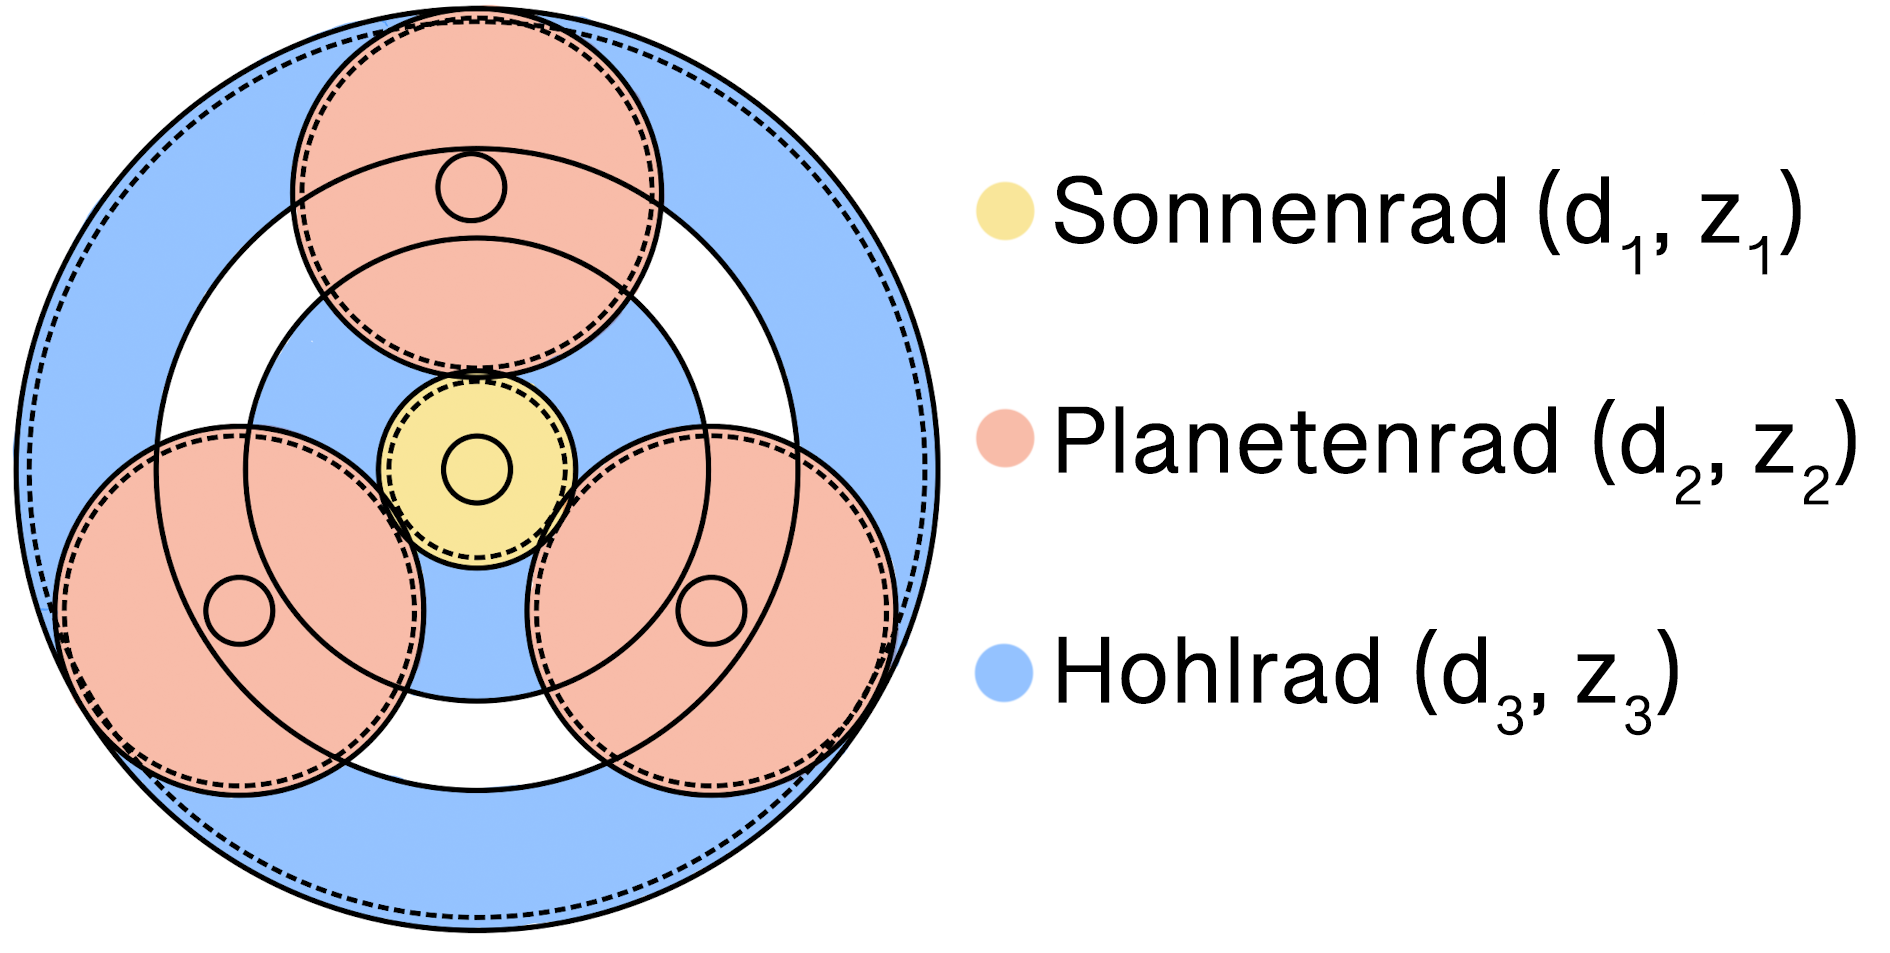
\includegraphics[width = 0.6\linewidth]{src/images/MAEIP_Planetenrad}
    \begin{footnotesize}
        \begin{center}
            \scriptsize{Innenverzahntes Rad besitzt per Definition negative Vorzeichen!}
            \begin{empheq}[box=\fbox]{align*}
                d_3 = 2\cdot d_2  + d_1 \quad &\mid \quad -z_3 = 2\cdot z_2 + z_1 \\
                \mathbb{Z} = \frac{|z_1| + |z_3|}{p} \quad &\mid \quad n_1 = (1-i_0)n_s +i_0n_3 \\
                i_0 = \frac{z_2}{z_1} \cdot \frac{z_3}{z_2} = \frac{n_1}{n_3} &= \frac{M_3}{M_1} = \frac{z_3}{z_1} = \frac{-d_3}{d_1}
            \end{empheq}
        \end{center}
    \end{footnotesize}
    \begin{scriptsize}
            $p = \text{Anzahl Planetenräder}; \; n_s = \text{Stegraddrehzahl}; \;i_0 = \text{Standübersetzung}$
    \end{scriptsize}
\par \vspace{1mm}\begin{center}
    \begin{footnotesize}
    \begin{tabular}{|c|c|c|c|}
        \hline
        An & Ab & Fest & $i(i_0 < 0)$\\
        \hline
        Sonne & Hohl & Steg & $i_0$\\
        \hline
        Hohl & Sonne & Steg & $1/i_0$\\
        \hline
        Sonne & Steg & Hohl & $1-i_0$\\
        \hline
        Steg & Sonne & Hohl & $1 / (1-i_0)$\\
        \hline
        Hohl & Steg & Sonne & $i_0 - (1/i_0)$\\
        \hline
        Steg & Hohl & Sonne & $i_0 / (i_0-1)$\\
        \hline 
     \end{tabular}
    \end{footnotesize}
\end{center}